\bigskip
Pour ce QCM, aucune justification n'est demandée. On en fournit quand même dans ce corrigé.
\begin{enumerate}
\item \textbf{Réponse B.}

$F$ est dérivable sur $\R $, en tant que produit de fonctions dérivables sur cet intervalle.

$F$ est de la forme $u \times v$ avec $u(x)=x-1$ et $v(x)=\mathrm{e}^x$

On a donc, pour tout réel $x$,  $u'(x)=1$ et $v'(x)	=\mathrm{e}^x$

$F= u'\times v + v'\times u$ donc,  pour tout réel $x$, $F'(x) = \mathrm{e}^x+ (x-1) \mathrm{e}^x = x\mathrm{e}^x=f(x)$ .

Donc $F$ est une primitive de $f$ sur $\R$.
\item \textbf{Réponse D.}

Par lecture graphique : $f(x)<0$ sur $]0~;~1[$ et $f(x)>0$ sur $]1~;~+\infty[$.

D'après l'énoncé : le maximum de la fonction $f$ est atteint au point d'abscisse 3  donc $f'(x)>0$ sur $]0~;~3[$ et $f'(x) <0$ sur $]3~;~+\infty[$.

D'après l'énoncé : le point d'abscisse 5 est le seul point d'inflexion, de plus,  par lecture  graphique,  la fonction est concave puis convexe donc : $f''(x)<0$ sur $]0~;~5[$ et $f''(x) >0$ sur $]5~;~+\infty[$.



Pour tout $x \in ]5~;~+\infty[$, $f(x)$ et $f''(x)$ sont de même signe.

\item \textbf{Réponse D.}

Pour tout réel positif $t$, $g(t)=\dfrac{a}{b+\mathrm{e}^{-t}}$.

D'une part  $g(0)=\dfrac{a}{b+\mathrm{e}^0}=\dfrac{a}{b+1}=2$ donc $\dfrac{a}{b+1}=2 \iff a=2(b+1)=2b+2$.

D'autre part :

$\lim\limits_{t \to +\infty}{-t}=-\infty$ et $\lim\limits_{X\to -\infty}{\mathrm{e}^X}=0$, donc, par composition, $\lim\limits_{t\to +\infty}{ \mathrm{e}^{-t}}=0$

d'où, par somme, $\lim\limits_{t\to +\infty} b+ \mathrm{e}^{-t}=b$

et donc, par quotient $\lim\limits_{t\to +\infty}\dfrac{a}{b+\mathrm{e}^{-t}}=\dfrac{a}{b}$

d'où $\dfrac{a}{b}=3 \Leftrightarrow a=3b$

On a donc $a=2b+2=3b$ d'où $b=2$ et $a=3\times 2=6$
\item \textbf{Réponse C.}

\begin{minipage}{9.5cm}
Soient:
	\begin{itemize}
	\item $A$ l'évènement \og Alice choisit l'urne A \fg
	\item $B$ l'évènement \og Alice choisit l'urne B \fg
	\item $V$ l'évènement \og Elle obtient une boule verte \fg
	\item $R$ l'évènement \og Elle obtient une boule rouge \fg
\end{itemize}

	La situation peut être représentée à l'aide de l'arbre ci-contre :
	\end{minipage}	\hfill
	

\begin{tikzpicture}[xscale=1,yscale=1,baseline=(R)]

\tikzstyle{fleche}=[->,>=latex,thick]
			\tikzstyle{noeud}=[fill=white,circle,inner sep=2pt]
			\tikzstyle{feuille}=[fill=white,circle,inner sep=2pt]
			\tikzstyle{etiquette}=[midway,fill=white, inner xsep=3pt, inner ysep=1.5pt]

\def\DistanceInterNiveaux{2}
\def\DistanceInterFeuilles{1}

\def\NiveauA{(0)*\DistanceInterNiveaux}
\def\NiveauB{(1.5)*\DistanceInterNiveaux}
\def\NiveauC{(2.5)*\DistanceInterNiveaux}
\def\InterFeuilles{(-1)*\DistanceInterFeuilles}

\node[noeud] (R) at ({\NiveauA},{(1.5)*\InterFeuilles}) {};
\node[noeud] (Ra) at ({\NiveauB},{(0.5)*\InterFeuilles}) {$A$};
\node[feuille] (Raa) at ({\NiveauC},{(0)*\InterFeuilles}) {$V$};
\node[feuille] (Rab) at ({\NiveauC},{(1)*\InterFeuilles}) {$R$};
\node[noeud] (Rb) at ({\NiveauB},{(2.5)*\InterFeuilles}) {$B$};
\node[feuille] (Rba) at ({\NiveauC},{(2)*\InterFeuilles}) {$V$};
\node[feuille] (Rbb) at ({\NiveauC},{(3)*\InterFeuilles}) {$R$};

\draw[fleche] (R.east)--(Ra) node[etiquette] {$\dfrac{1}{2}$};
\draw[fleche] (Ra.east)--(Raa) node[etiquette,pos=0.45] {$\frac{1}{2}$};
\draw[fleche] (Ra.east)--(Rab) node[etiquette,pos=0.65] {$\frac{1}{2}$};
\draw[fleche] (R.east)--(Rb) node[etiquette] {$\dfrac{1}{2}$};
\draw[fleche] (Rb.east)--(Rba) node[etiquette,pos=0.45] {$\frac{3}{4}$};
\draw[fleche] (Rb.east)--(Rbb) node[etiquette,pos=0.65] {$\frac{1}{4}$};
\end{tikzpicture}


On cherche la probabilité $P_V(B)$.

$P(\mathrm{V} \cap B) = P(B) \times P_ B(V)=\dfrac{1}{2}\times \dfrac{3}{4}=\dfrac{3}{8}$

Les évènements $A$ et $B$ partitionnant l'univers,  la loi des probabilités totales donne :

$P(V)=P(V\cap A )+p(V \cap B) =P(A) \times P_A(V) +\dfrac{3}{8}=\dfrac{1}{2}\times \dfrac{1}{2}+\dfrac{3}{8}=\dfrac{1}{4}+\dfrac{3}{8}= \dfrac{2}{8}+\dfrac{3}{8}=\dfrac{5}{8}$

$P_V(B)=\dfrac{P(V\cap B)}{P(V)}= \dfrac{\frac{3}{8}}{\frac{5}{8}}= \dfrac{3}{5}$.
\item \textbf{Réponse B.}








On cherche l'algorithme qui permet de calculer la somme des 100 premiers termes de la suite $\left( u_n\right)$ définie sur $\N$ par $u_n=\dfrac{1}{n}$.
	
	L'algorithme A.  calcule chaque terme mais ils ne sont pas additionnés,  ce n'est pas la réponse A. 
	
	L'algorithme C.  initialise le compteur k,  il ne peut donc pas comparer S à 100,  l'algorithme ne fonctionne pas,  ce n'est pas la réponse C.

	L'algorithme D. initialise le compteur k à zéro mais il n'est pas incrémenté dans la boucle while,  k faudra toujours 0 et l'algorithme ne s'arrête jamais, ce n'est donc pas l'algorithme D. 

	Par élimination,  c'est donc l'algorithme B. 

\end{enumerate}
\bigskip
